

    \item A uniform magnetic field \textbf{B} exists in the region between \(x = 0\) and \(x = \frac{3R}{2}\) (region 2 in the figure) pointing normally into the plane of the paper. A particle with charge \(+Q\) and momentum \textbf{p} directed along x-axis enters region 2 from region 1 at point \(P_1\) (\(y = -R\)). Which of the following option(s) is/are correct?
        \begin{tasks}(1)
            \task For \(B \geq \frac{2}{3} \frac{p}{qR}\), the particle will re-enter region 1
            \task For \(B = \frac{8}{13} \frac{p}{qR}\), the particle will enter region 3 through the point \(P_2\) on x-axis
            \task When the particle re-enters region 1 through the longest possible path in region 2, the magnitude of the change in its linear momentum between point \(P_1\) and the farthest point from y-axis is \(p\sqrt{2}\)
            \task For a fixed \(B\), particles of same charge \(Q\) and same velocity \(v\), the distance between the point \(P_1\) and the point of re-entry into region 1 is inversely proportional to the mass of the particle
        \end{tasks}

\begin{center}
    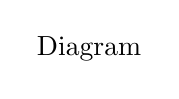
\begin{tikzpicture}
        \node {Diagram};
    \end{tikzpicture}
\end{center}
